\documentclass[a4paper,12pt]{extarticle}
\usepackage{geometry}
\usepackage[T2A,T1]{fontenc}
\usepackage[utf8]{inputenc}
\usepackage[russian,main=english]{babel}
\usepackage{amsmath}
\usepackage{amsthm}
\usepackage{amssymb}
\usepackage{fancyhdr}
\usepackage{setspace}
\usepackage{graphicx}
\usepackage{colortbl}
\usepackage{tikz}
\usepackage{pgf}
\usepackage{subcaption}
\usepackage{listings}
\usepackage{indentfirst}
\usepackage[
backend=biber,
style=numeric,
maxbibnames=99
]{biblatex}
\addbibresource{refs.bib}
\usepackage[colorlinks,citecolor=blue,linkcolor=blue,bookmarks=false,hypertexnames=true, urlcolor=blue]{hyperref} 
\usepackage{indentfirst}
\usepackage{mathtools}
\usepackage{booktabs}
\usepackage[flushleft]{threeparttable}
\usepackage{tablefootnote}

\usepackage{chngcntr} % нумерация графиков и таблиц по секциям
\counterwithin{table}{section}
\counterwithin{figure}{section}

\graphicspath{{graphics/}}%путь к рисункам

\makeatletter
% \renewcommand{\@biblabel}[1]{#1.} % Заменяем библиографию с квадратных скобок на точку:
\makeatother

\geometry{left=2.5cm}% левое поле
\geometry{right=1.0cm}% правое поле
\geometry{top=2.0cm}% верхнее поле
\geometry{bottom=2.0cm}% нижнее поле
\setlength{\parindent}{1.25cm}
\renewcommand{\baselinestretch}{1.5} % междустрочный интервал

\AtBeginDocument{
  \renewcommand{\figurename}{Figure}
  \renewcommand{\tablename}{Table}
}

\selectlanguage{english}

\newcommand{\bibref}[3]{\hyperlink{#1}{#2 (#3)}} % biblabel, authors, year
\addto\captionsrussian{\def\refname{Список литературы (или источников)}} 

\renewcommand{\theenumi}{\arabic{enumi}}% Меняем везде перечисления на цифра.цифра
\renewcommand{\labelenumi}{\arabic{enumi}}% Меняем везде перечисления на цифра.цифра
\renewcommand{\theenumii}{.\arabic{enumii}}% Меняем везде перечисления на цифра.цифра
\renewcommand{\labelenumii}{\arabic{enumi}.\arabic{enumii}.}% Меняем везде перечисления на цифра.цифра
\renewcommand{\theenumiii}{.\arabic{enumiii}}% Меняем везде перечисления на цифра.цифра
\renewcommand{\labelenumiii}{\arabic{enumi}.\arabic{enumii}.\arabic{enumiii}.}% Меняем везде перечисления на цифра.цифра

% Set up font encoding switching
\DeclareTextFontCommand{\textcyr}{\fontencoding{T2A}\selectfont}

\begin{document}
% Switch to T2A encoding for the title page which contains Cyrillic
{\fontencoding{T2A}\selectfont
\begin{titlepage}
\newpage

\begin{center}
FEDERAL STATE AUTONOMOUS EDUCATIONAL INSTITUTION FOR\\
HIGHER PROFESSIONAL EDUCATION NATIONAL RESEARCH\\
UNIVERSITY\\
«HIGHER SCHOOL OF ECONOMICS»\\
\bigskip
Faculty of Computer Science
\end{center}

\vspace{2em}

\begin{center}
\underline{Marozau Leu}
\end{center}

\vspace{2em}

\begin{center}
Обнаружение эмоций на основе текста
\end{center}

\vspace{2em}

\begin{center}
Text-Based Emotion Detection
\end{center}

\vspace{4em}

\begin{center}
Qualification paper — Master of Science Dissertation\\
Field of study 01.04.02 «Applied Mathematics and Informatics»\\
Program: 
\end{center}

\vspace{6em}

\begin{flushleft}
Student\\
Marozau Leu
\end{flushleft}

\vspace{4em}

\begin{flushright}
Supervisor\\
Shirnin Alexander Andreevich
\end{flushright}

\vspace{\fill}

\begin{center}
Moscow, 2025
\end{center}

\end{titlepage}

}
\newpage
\setcounter{page}{2}

% Switch back to T1 encoding for the rest of the document
\fontencoding{T1}\selectfont
\selectlanguage{english}

{
	\hypersetup{linkcolor=black}
	\tableofcontents
}

\newpage

\section*{Abstract}

This thesis explores various approaches for multi-label emotion detection in text across multiple languages. 
We investigate traditional supervised approaches including BERT, SetFit, and Seq2Seq models, as well as a novel retrieval-augmented generation system called EmoRAG. 
Using the BRIGHTER dataset, which covers 28 languages including many low-resource ones, we demonstrate that our EmoRAG system achieves state-of-the-art performance without requiring extensive model training. 
Notably, our EmoRAG system participated in the SemEval2025-Task11: "Bridging the Gap in Text-Based Emotion Detection" competition, achieving top-10 average performance across all languages, with many languages ranking in the top-3 positions. 
Our paper describing the EmoRAG system has been accepted for presentation at the ACL Workshop 2025. The complete implementation of our system is available in our open-source repository at \url{https://github.com/galthran-wq/semeval25-text-emotions}.

\addcontentsline{toc}{section}{Abstract}

\section*{Keywords}
Deep learning, emotion detection, multilingual NLP, retrieval-augmented generation, low-resource languages, multi-label classification

\section{Introduction}

Emotions are fundamental to human communication and experience, coloring our interactions, decisions, and perceptions. The ability to detect and understand emotions in text has become increasingly important in natural language processing (NLP), with applications spanning various domains including customer service, mental health monitoring, content recommendation, social media analysis, and educational technology.

Unlike traditional sentiment analysis, which typically focuses on determining whether a text is positive, negative, or neutral, emotion detection aims to identify specific emotional states such as joy, sadness, anger, fear, surprise, and disgust. This fine-grained understanding of affective content enables more nuanced and human-like interactions between computational systems and users.

The development of effective multi-lingual, multi-label emotion detection systems faces several interconnected challenges. Linguistic diversity presents a significant hurdle, as human languages vary dramatically in their lexical, syntactic, and semantic structures, including how emotions are expressed. Data scarcity is particularly problematic for low-resource languages, which lack substantial labeled datasets for emotion detection. The multi-label nature of emotions adds complexity, as texts frequently express multiple emotions simultaneously. Cross-cultural variations in how emotions are expressed and interpreted further complicate the development of universally applicable systems. Finally, computational efficiency concerns arise when considering the impracticality of training separate models for thousands of languages.

This thesis investigates multi-lingual, multi-label emotion detection, exploring approaches that can operate effectively with limited labeled data, adapt to linguistic and cultural differences, and handle the inherent complexity of multi-label emotion classification. We compare traditional supervised approaches with newer paradigms like retrieval-augmented generation, examining their effectiveness across languages with varying resource availability.

The remainder of this thesis is organized as follows:

\textbf{Chapter 2: Related Work} reviews previous research in emotion detection, multi-label classification, multi-lingual NLP models, retrieval-augmented generation, few-shot learning, and large language models for emotion detection.

\textbf{Chapter 3: Data} describes the BRIGHTER dataset, including its creation, annotation process, and composition.

\textbf{Chapter 4: Methodology} presents our four approaches: BERT-based fine-tuning, SetFit few-shot learning, Seq2Seq generative models, and our novel EmoRAG system.

\textbf{Chapter 5: Experiments} outlines our experimental setup, evaluation metrics, and hyperparameter tuning strategies.

\textbf{Chapter 6: Ablation Studies} presents ablation studies of the EmoRAG system, examining the impact of different components on performance.

\textbf{Chapter 7: Results} analyzes our experimental findings, including performance comparisons across approaches, languages, and emotion categories.

\textbf{Chapter 8: Discussion} interprets our results, comparing the strengths and weaknesses of each approach.

\textbf{Chapter 9: Conclusions} summarizes key findings and suggests directions for future research.

\section{Related Work}

This chapter reviews key literature relevant to multi-lingual, multi-label emotion detection, focusing on four areas: traditional approaches to emotion detection, multi-label classification techniques, large language models, and retrieval-augmented generation systems.

\subsection{Emotion Detection in Text}

Emotion detection in text has evolved significantly over the past two decades. Early work by \cite{strapparava2007semeval} introduced one of the first datasets for emotion recognition in English text, defining the task as detecting Ekman's six basic emotions: joy, sadness, anger, fear, surprise, and disgust. This work established the foundation for most subsequent research in the field.

Classical approaches to emotion detection included lexicon-based methods and traditional machine learning techniques. \cite{mohammad2013crowdsourcing} developed the NRC Emotion Lexicon, mapping English words to emotions. These approaches provide strong baselines but struggle with contextual understanding and required extensive manual annotation for each language.

The advent of deep learning brought significant advances to emotion detection. \cite{felbo2017using} introduced DeepMoji, leveraging distant supervision from emojis to pre-train models for emotion recognition. More recently, transformer-based approaches have set new benchmarks. \cite{demszky2020goemotions} created GoEmotions, a large-scale dataset with 27 emotion categories, and demonstrated strong performance with BERT-based models.

\subsection{Multi-label Classification and Language Models}

Multi-label classification, where instances can belong to multiple categories simultaneously, is inherently relevant to emotion detection as texts often express multiple emotions at once. 

Classical approaches to multi-label classification include binary relevance, which trains independent classifiers for each label, and label powerset, which transforms the problem into a multi-class classification task with each unique label combination as a separate class. \cite{read2011classifier} introduced classifier chains, which model inter-label dependencies by building a sequence of binary classifiers, demonstrating significant improvements over binary relevance methods.

The evolution of language models has dramatically impacted text classification tasks, including emotion detection. BERT \cite{devlin2019bert} and its multilingual variant mBERT demonstrated strong performance across languages and tasks through contextual representations and pre-training on massive corpora. XLM-RoBERTa \cite{conneau2020unsupervised} further improved cross-lingual capabilities by training on 100 languages with 2.5 times more data than mBERT.

Large Language Models (LLMs) like GPT-3 \cite{brown2020language} and its successors have shown remarkable few-shot capabilities through in-context learning, where models make predictions based on examples provided in the prompt. This paradigm shift has significant implications for multi-lingual emotion detection, potentially reducing the need for extensive labeled data in each language.

For multi-label settings, deep learning approaches have shown promise. \cite{nam2014large} demonstrated that using cross-entropy loss with a sigmoid activation function per label outperforms ranking-based loss functions in neural networks. 

\subsection{Few-shot Learning in NLP}

Few-shot learning has become increasingly important for addressing data scarcity in NLP, particularly for low-resource languages. \cite{brown2020language} demonstrated the remarkable few-shot capabilities of large language models through in-context learning, where a model makes predictions based on a few examples provided in the prompt.

Building on this foundation, \cite{gao2021making} showed that carefully constructed prompts with strategically selected examples can dramatically improve few-shot performance on various NLP tasks, including classification. For more specialized applications, \cite{tunstall2022efficient} developed SetFit, a few-shot learning approach that combines contrastive learning with classification fine-tuning. By leveraging sentence transformers and efficient pair-wise training, SetFit achieves strong performance with as few as 8 examples per class.

The selection of examples for few-shot learning significantly impacts performance. \cite{liu2022few} showed that retrieving examples based on semantic similarity to the test instance outperforms random selection, especially for complex tasks. Cross-lingual few-shot learning presents additional challenges. 

Despite these advances, few-shot learning in multi-label settings remains challenging. \cite{hou2022few} addressed this gap with a specialized few-shot learning approach for multi-label classification that captures label correlations even with limited examples.

\subsection{Retrieval-Augmented Generation (RAG)}

Retrieval-Augmented Generation (RAG) has emerged as a powerful paradigm for enhancing language model capabilities with external knowledge. \cite{lewis2020retrieval} introduced the original RAG framework, combining dense retrieval with sequence-to-sequence models to generate outputs conditioned on relevant retrieved documents.

While RAG was initially developed for generation tasks, its application to classification has shown promising results. \cite{gao2024retrieval} adapted RAG for text classification, demonstrating that retrieved examples can serve as few-shot demonstrations to guide in-context learning. Their approach achieved competitive performance on various classification benchmarks without requiring task-specific fine-tuning.

For multi-lingual contexts, \cite{shi2023replug} developed Cross-Lingual RAG, which leverages a shared dense retrieval space across languages to retrieve relevant documents for low-resource languages. This approach is particularly valuable for emotion detection across diverse languages, as it enables knowledge transfer from high-resource to low-resource languages.

The selection of retrieved documents significantly impacts RAG performance. \cite{gao2023retrieval} introduced techniques for dynamic retrieval that adapt to the specific needs of each query, showing that adaptive retrieval strategies outperform static approaches. In classification contexts, \cite{singh2022flare} demonstrated that RAG can mitigate the challenge of domain shift by retrieving examples similar to the test instance, regardless of their source domain.

\subsection{Research Gaps and Opportunities}

Our review of the literature reveals several important gaps that this thesis aims to address:

\begin{enumerate}

    \item \textbf{Few-shot Learning for Low-resource Languages}: Most emotion detection systems require substantial labeled data, which is unavailable for many languages. Few studies have explored how large language models can effectively perform emotion detection with minimal examples across diverse languages.
    
    \item \textbf{Ensemble Methods for Multi-label Emotion Detection}: While ensemble approaches have shown promise in various NLP tasks, their application to multi-label emotion detection, particularly in multi-lingual settings, remains underexplored. There is limited research on how to effectively combine multiple LLM predictions to improve performance across emotions and languages.
    
    \item \textbf{Retrieval-Augmented Classification}: While RAG has shown promise for generation tasks, its application to multi-label classification, particularly emotion detection, remains underexplored.

    \item \textbf{Balancing Performance Across Languages}: Existing approaches often show significant performance disparities between high-resource and low-resource languages. Few studies have systematically addressed how to design systems that maintain consistent performance across linguistically diverse languages.
    
    \item \textbf{Low-Resource Adaptability}: Few studies have explicitly addressed how emotion detection approaches can be adapted for low-resource languages with minimal labeled data.

    \item \textbf{Capturing Emotion Co-occurrence Patterns}: The multi-label nature of emotion detection presents unique challenges, as emotions often co-occur in complex patterns. Limited research exists on how few-shot LLM approaches can effectively model these interdependencies without extensive training data.
    
\end{enumerate}

\section{Data}
\subsection{Overview}

\begin{figure}[h]
    \centering
    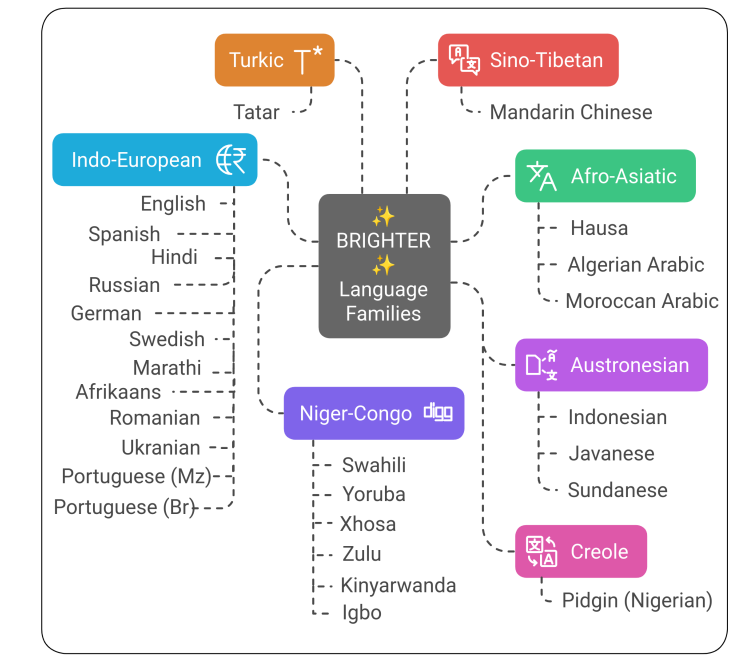
\includegraphics[width=0.5\textwidth]{brighter_languages.png}
    \caption{Languages in the BRIGHTER dataset}
    \label{fig:brighter_languages}
\end{figure}

\begin{figure}[h]
    \centering
    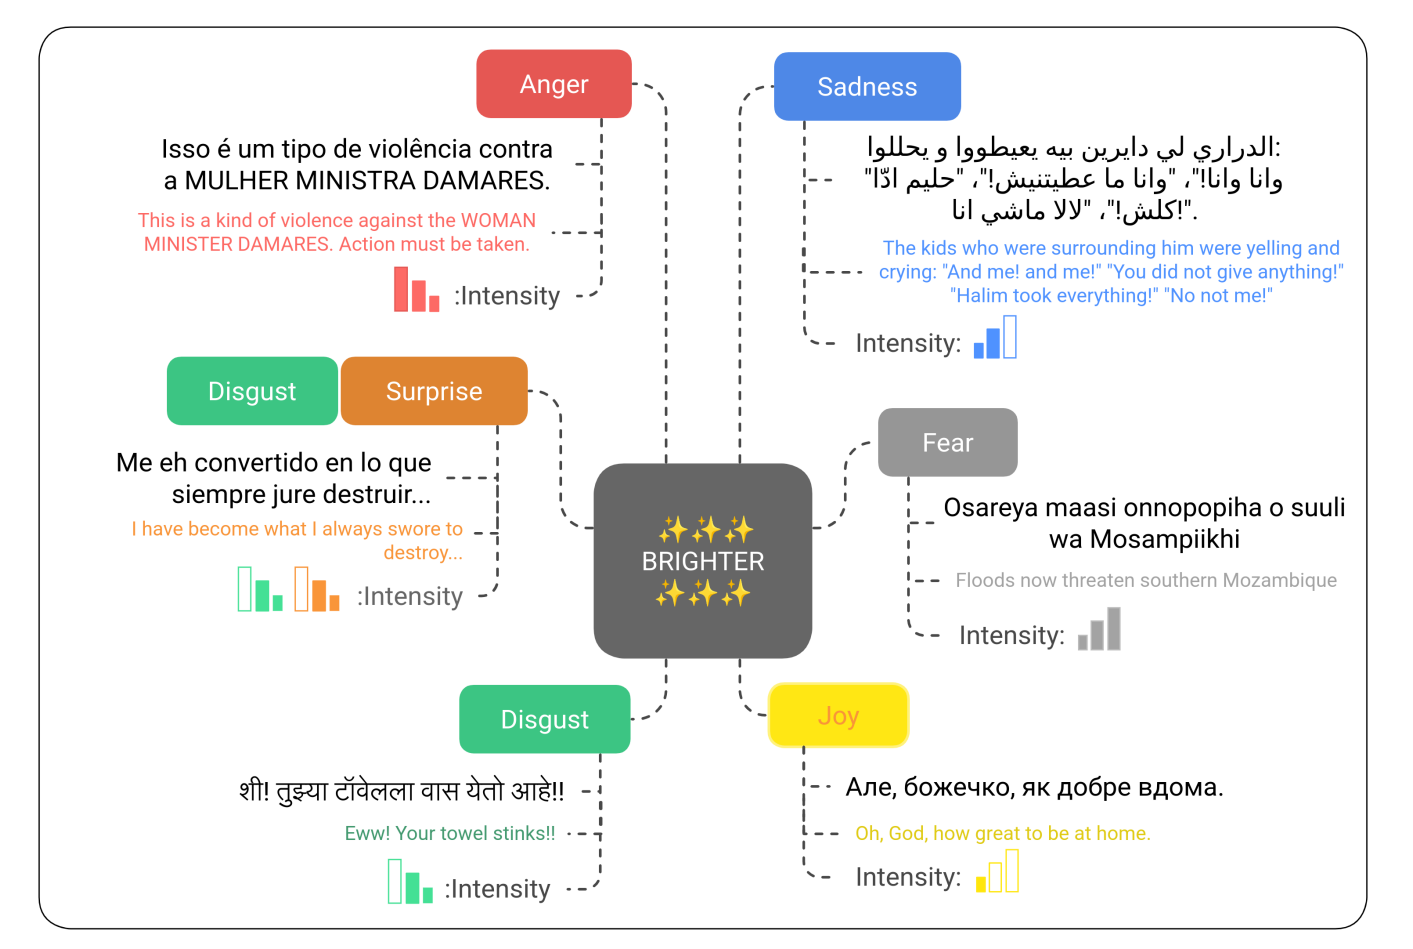
\includegraphics[width=0.8\textwidth]{brighter_examples.png}
    \caption{Examples from the BRIGHTER dataset}
    \label{fig:brighter_examples}
\end{figure}

The BRIGHTER dataset \cite{muhammad2025brighterbridginggaphumanannotated} is a comprehensive, multi-labeled, multilingual resource for textual emotion recognition, consisting of over 100,000 annotated examples across 28 languages and 7 language families. Designed to address the stark resource imbalance in emotion research, BRIGHTER prioritizes low-resource languages from Africa, Asia, Eastern Europe, and Latin America, while also including mid- and high-resource languages such as English, German, and Portuguese.

Each instance in BRIGHTER is manually annotated by fluent speakers, with annotations covering six core perceived emotions — \textit{joy}, \textit{sadness}, \textit{anger}, \textit{fear}, \textit{surprise}, and \textit{disgust} — and includes an additional \textit{neutral} label when no emotion is expressed. Annotations are multi-label and span four emotion intensity levels (0 to 3).

The dataset aggregates data from diverse sources, including social media platforms (e.g., Reddit, YouTube, Weibo), speeches, literature, news, and even machine-generated examples with human post-editing. A detailed breakdown of these sources, annotator counts, and splits per language is given in the original BRIGHTER paper, with representative examples shown in Figure~\ref{fig:brighter_examples} and the language family distribution illustrated in Figure~\ref{fig:brighter_languages}.

\subsection{Data Splits}
We use the official BRIGHTER dataset splits for all experiments. The Training Set comprises approximately 70\% of the data and is used for supervised model training. The Validation Set, which makes up about 15\% of the data, is utilized for early stopping and hyperparameter tuning. Finally, the Test Set also consists of approximately 15\% of the data and is reserved for final evaluation.

\subsection{Dataset Challenges}

\begin{figure}[h]
    \centering
    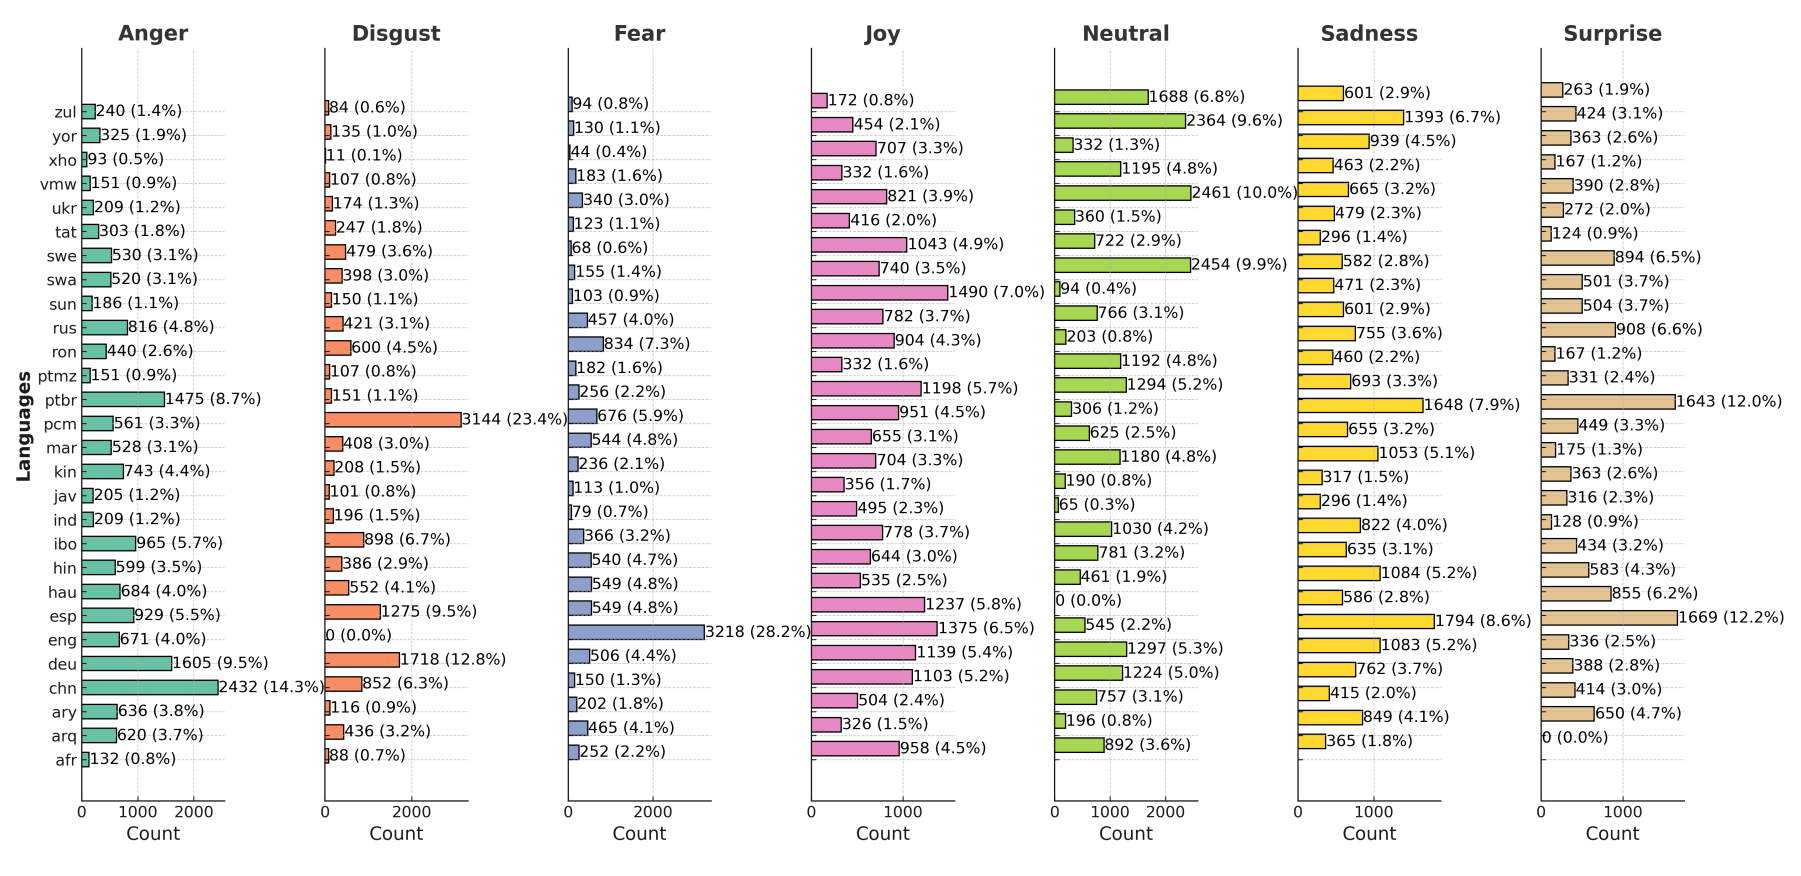
\includegraphics[width=1\textwidth]{brighter_label_distribution.png}
    \caption{Label distribution in the BRIGHTER dataset}
    \label{fig:brighter_label_distribution}
\end{figure}

While BRIGHTER is a rich and diverse resource, it also introduces several challenges that motivated our modeling choices:

Label Distribution: The dataset exhibits long-tailed distributions for both emotions and languages, as illustrated in Figure~\ref{fig:brighter_label_distribution}. Some languages lack examples for certain emotions (e.g., no \textit{disgust} in English, no \textit{surprise} in Afrikaans), and neutral examples vary greatly in frequency.

Linguistic Coverage: BRIGHTER spans typologically diverse languages with varying scripts (Latin, Arabic, Devanagari, Cyrillic), making it a strong benchmark for cross-lingual generalization.

Annotation Density: Most languages have between 3 and 10 annotators per example, but annotation intensity and agreement levels vary. Final labels were aggregated using a combination of per-emotion thresholding and average intensity, ensuring consistent quality across languages.

These considerations led us to explore both supervised and retrieval-augmented methods, with the aim of improving generalization under low-resource, high-diversity conditions.

\section{Methodology}

This chapter presents the various approaches we explored for multi-lingual, multi-label emotion detection using the BRIGHTER dataset. We investigate both traditional supervised learning approaches (BERT, SetFit, and Seq2Seq) and a novel retrieval-augmented generation (RAG) approach called EmoRAG. Each approach represents a different paradigm in machine learning for text classification:

\begin{enumerate}
\item \textbf{BERT-based Approach}: Fine-tune a pre-trained language model with a classification head for multi-label prediction
\item \textbf{SetFit Approach}: A few-shot learning technique that combines contrastive learning with standard classification techniques
\item \textbf{Seq2Seq Approach}: Framing emotion detection as a text generation task
\item \textbf{EmoRAG System}: A novel retrieval-augmented generation system that leverages few-shot learning without parameter updates
\end{enumerate}

The following sections describe each approach in detail, including model architecture, training procedures, and implementation specifics.

\subsection{BERT-based Approach}

For prediction, we apply a sigmoid function to the model outputs and use a threshold of 0.5 to convert probabilities to binary predictions:

The BERT-based approach provides a strong baseline for emotion detection, leveraging the powerful contextual representations of transformer models. However, it may struggle with low-resource languages where pre-training data is limited.

\subsection{Seq2Seq Approach}

The Seq2Seq approach reframes multi-label emotion detection as a text generation task, where the model generates a comma-separated list of emotions present in the input text. This approach leverages the generative capabilities of encoder-decoder transformer models to directly produce structured outputs rather than independent binary classifications.

This approach is particularly interesting because of the large number of available pre-trained encoder-decoder models.

Some examples of pre-trained encoder-decoder models are:

\textbf{mT5} \cite{xue2021mt5massivelymultilingualpretrained}: A multilingual variant of T5 (Text-to-Text Transfer Transformer) pre-trained on 101 languages. 

\textbf{BART} \cite{lewis2019bartdenoisingsequencetosequencepretraining}: A denoising autoencoder for pretraining sequence-to-sequence models. 

\textbf{mBART} \cite{liu2020multilingualdenoisingpretrainingneural}: A multilingual sequence-to-sequence denoising auto-encoder pre-trained on 25 languages.

The Seq2Seq approach transforms the multi-label classification problem into a text generation task:

\textbf{Input}: The original text to be classified. 

\textbf{Output}: A comma-separated list of emotion labels present in the text (e.g., "joy,surprise,fear").

This format allows the model to learn the relationships between emotions naturally through the generation process, potentially capturing label co-occurrences and dependencies more effectively than independent binary classifiers.

\subsection{SetFit Approach}

SetFit (Sentence Transformer Fine-tuning) is a novel few-shot learning method introduced by \cite{tunstall2022efficient} that combines contrastive learning with standard classification techniques. It was designed to achieve strong performance with limited labeled data, making it particularly suitable for multi-lingual emotion detection where labeled examples may be scarce for low-resource languages.

The SetFit approach involves two stages. 

The first stage is the \textbf{Contrastive Learning Stage}, where a sentence transformer model is fine-tuned using contrastive learning on sentence pairs derived from labeled examples. 

The second stage is the \textbf{Classification Stage}, where a classifier, typically a linear model, is trained on the embeddings produced by the fine-tuned sentence transformer.

Figure~\ref{fig:setfit_training} illustrates the SetFit training process.

\begin{figure}[h]
    \centering
    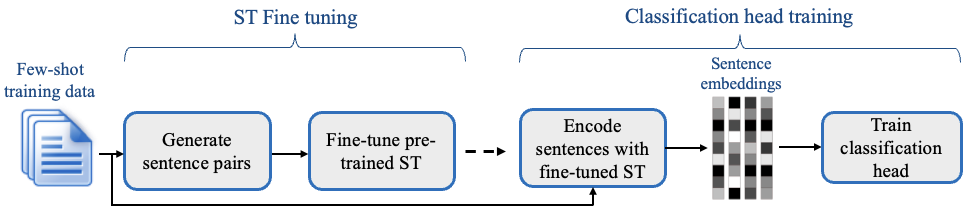
\includegraphics[width=0.8\textwidth]{setfit.png}
    \caption{SetFit training process}
    \label{fig:setfit_training}
\end{figure}

The key innovation of SetFit is its ability to leverage the power of sentence transformers for few-shot learning without requiring extensive labeled data or computationally expensive prompt-based approaches. By fine-tuning the sentence embeddings directly on the task-specific data, SetFit can adapt pre-trained embeddings to better represent the nuances of emotion detection across languages.

\subsection{EmoRAG System}

EmoRAG (Emotion Retrieval-Augmented Generation) is a novel system developed for multi-label emotion detection that reframes the problem through the lens of retrieval-augmented generation. Rather than relying on model fine-tuning, EmoRAG leverages the knowledge captured in labeled examples retrieved at inference time, enabling multilingual, few-shot emotion classification without updating model parameters.

\subsubsection{Pipeline Overview}

The EmoRAG architecture follows a four-stage pipeline, illustrated in Figure~\ref{fig:emorag_pipeline}:

\begin{enumerate}
\item \textbf{Database Construction}: The system first indexes the labeled examples from the BRIGHTER training dataset as a retrieval corpus.
\item \textbf{Retrieval}: An n-gram or embedding-based retriever fetches the top-K most similar examples to a given input.
\item \textbf{Generation}: The retrieved examples are used as few-shot prompts for a set of pre-trained large language models (LLMs) to produce emotion predictions.
\item \textbf{Aggregation}: The individual model predictions are combined via a learned or heuristic aggregation strategy (e.g., majority vote, label-weighted averaging) to produce the final multi-label output.
\end{enumerate}


\begin{figure}[h]
    \centering
    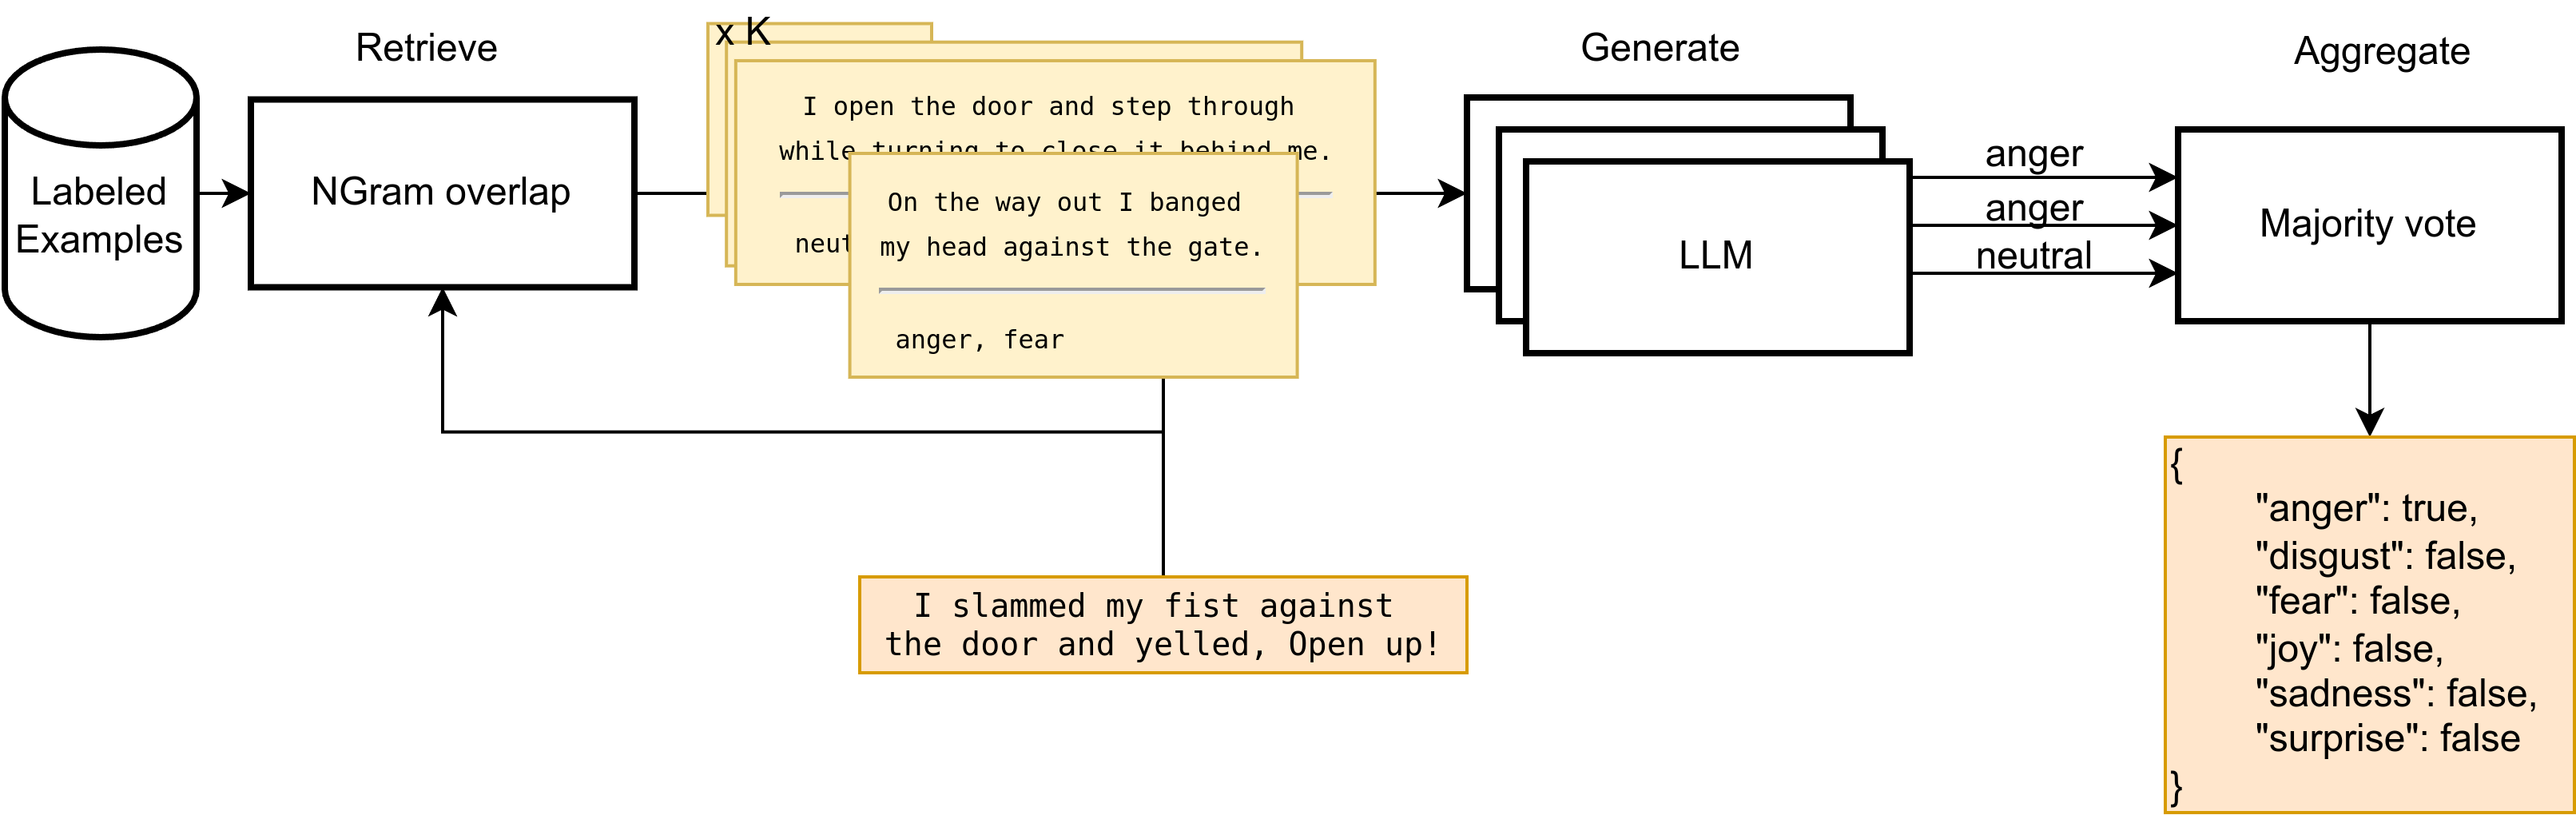
\includegraphics[width=0.8\textwidth]{emorag.png}
    \caption{The EmoRAG pipeline includes a retriever, a set of LLMs, and an aggregation module. Retrieved labeled examples are used as prompts to generate multi-label predictions.}
    \label{fig:emorag_pipeline}
\end{figure}

\subsubsection{Retriever Component}

We experimented with two retrieval strategies:


\textbf{N-gram Overlap}: Particularly effective for low-resource languages, this method retrieves examples based on surface lexical similarity. We have used the n-gram retriever from the 
\texttt{LangChain module}~\footnote{\href{https://python.langchain.com/docs/how_to/example_selectors_ngram}{\texttt{python.langchain.com}}}~\cite{Chase_LangChain_2022}. 


\textbf{Embedding-based Retrieval}: A dense vector retriever using sentence-level embeddings that supports multilingual representations. For our experiments, we used the BGE-M3 embedding model \cite{chen2024bgem3embeddingmultilingualmultifunctionality}, which achieved state-of-the-art performance on the multilingual subset of the MTEB benchmark \cite{muennighoff2023mtebmassivetextembedding}.

The number of retrieved samples K is fixed per language type: 30 for low-resource languages and 100 for high-resource ones.

\subsubsection{Generator Models}

For generation, EmoRAG uses a diverse ensemble of LLMs including:
\texttt{Llama-3.1-70B \cite{grattafiori2024llama3herdmodels}}, \texttt{Qwen2.5-72B-Instruct \cite{yang2024qwen2technicalreport}}, \texttt{Gemma-2-27B-it \cite{gemmateam2024gemma2improvingopen}}, \texttt{GPT-4o-mini \cite{openai2024gpt4omini}}
Each LLM receives the same prompt structure, written in English and formatted to generate emotion predictions in JSON format:
\begin{verbatim}
{
"anger": bool,
"fear": bool,
"joy": bool,
"sadness": bool,
"surprise": bool,
"disgust": bool
}
\end{verbatim}

\subsubsection{Aggregation Strategies}

To aggregate predictions from multiple LLMs, we evaluate five strategies. 

The \textbf{Single model} approach simply uses predictions from one LLM (e.g., GPT-4o-mini) without any aggregation. 

\textbf{Majority Vote} gives each model an equal vote for each emotion label, with the final prediction determined by the majority decision (threshold > 0.5). 

In \textbf{Macro/Micro-F1 Weighted Voting}, models' votes are weighted by their macro or micro F1 scores on the validation set for the specific language, giving more influence to better-performing models. 

\textbf{Label-specific F1 Voting} weights each model's vote by its F1 score for the specific emotion label and language, allowing models with higher performance on particular emotions to have more influence on those predictions. 

Finally, \textbf{LLM-based Aggregation} uses one LLM to analyze and aggregate the outputs from other models, potentially capturing more nuanced patterns in the predictions.

\section{Experiments}

\subsection{Experimental Setup}

Our experiments were conducted in two phases: first, a comprehensive evaluation of all approaches on English data to establish baseline performance, followed by an extensive multilingual evaluation focusing on our EmoRAG system across all 28 languages in the BRIGHTER dataset.

\subsubsection{Computing Infrastructure}

All experiments were conducted on the HSE University High-Performance Computing (HPC) Cluster "cHARISMa". This infrastructure provided essential computational resources for our large-scale experiments, particularly for training and evaluating transformer-based models. The cluster includes specialized nodes with NVIDIA Tesla V100 32GB GPUs and newer nodes with NVIDIA A100 80GB GPUs, which were crucial for training our larger models. For the most computationally intensive experiments, we utilized Type C computing nodes equipped with 4 NVIDIA Tesla V100 32GB GPUs with NVLink and 768GB RAM.

\subsubsection{Model Configurations}

For each approach, we employed the following configurations:

\begin{itemize}
\item \textbf{BERT-based Approach}: We fine-tuned XLM-RoBERTa-large (550M parameters) with a classification head for multi-label prediction. The model was initialized with pre-trained weights and fine-tuned on our emotion detection task with a learning rate of 2e-5 and batch size of 16.

\item \textbf{SetFit Approach}: We used the multilingual MPNet base model as our sentence transformer backbone, with a multi-output classification strategy. For few-shot learning, we sampled 8 examples per emotion category, balanced across languages when possible.

\item \textbf{Seq2Seq Approach}: We employed mT5-large (1.2B parameters) as our primary sequence-to-sequence model, fine-tuned with a learning rate of 5e-5 and a batch size of 8. We used a maximum sequence length of 512 tokens for both input and output.

\item \textbf{EmoRAG System}: Our retrieval component used the BGE-M3 embedding model for dense retrieval and n-gram retrieval, with K=30 for low-resource languages and K=100 for high-resource languages. The generator ensemble included Llama-3.1-70B, Qwen2.5-72B-Instruct, Gemma-2-27B-it, and GPT-4o-mini.
\end{itemize}

\subsubsection{Training Process}

For the supervised approaches (BERT, SetFit, and Seq2Seq), we trained models for 10 epochs with early stopping based on validation loss. The BERT and Seq2Seq models were trained using AdamW optimizer with a linear learning rate scheduler and 10\% warmup steps. 
For SetFit, we used a two-stage training process: contrastive learning followed by classifier training.

The EmoRAG system required no training in the traditional sense, as it leverages pre-trained models and retrieval mechanisms. 

All training runs were managed using the Slurm workload manager on the HPC cluster, with typical training times ranging from 2 hours for SetFit to 24 hours for the Seq2Seq approach on the full dataset.

For the English-only experiments, we used validation set for evaluation of different approaches.

Then, for EmoRAG system we provide evaluation both on the validation and test sets.

\subsection{Evaluation Metrics}

Our primary evaluation metrics were F1-micro and F1-macro scores, which are particularly suitable for multi-label classification tasks:

\textbf{F1-micro} calculates metrics globally by counting the total true positives, false negatives, and false positives across all instances. This metric gives equal weight to each sample and is therefore influenced more by common labels and high-resource languages.

\textbf{F1-macro} calculates metrics for each label separately and then takes the unweighted mean. This gives equal importance to each label regardless of its frequency, making it more suitable for evaluating performance on imbalanced datasets.

\section{Results}

\subsection{English Language}

Our experiments revealed significant performance differences across the various approaches to emotion detection. Table \ref{tab:english_comparison} presents a comprehensive comparison of all methods on the English subset of the BRIGHTER dataset.

\begin{table}[h]
\centering
\begin{tabular}{lcc}
\toprule
\textbf{Method} & \textbf{F1-micro} & \textbf{F1-macro} \\
\midrule
BERT (bert-large-cased) & 0.7145 & 0.6468 \\
SetFit (bge-m3) & 0.6943 & 0.5591 \\
Seq2Seq (bart-large-cnn) & 0.5126 & 0.4566 \\
GPT-4 (zero-shot) & 0.5959 & 0.6164 \\
\midrule
\multicolumn{3}{c}{\textbf{EmoRAG Variants}} \\
\midrule
Llama-3.1-70B (few-shot, bge-m3) & 0.7499 & 0.7239 \\
Qwen2.5 (few-shot, bge-m3) & 0.7790 & 0.7749 \\
GPT-4o-mini (few-shot, bge-m3) & 0.8071 & 0.8026 \\
GPT-4o-mini (few-shot, ngram) & 0.7810 & 0.7700 \\
EmoRAG (majority vote) & 0.8080 & 0.8010 \\
EmoRAG (majority vote macro) & 0.8130 & 0.8100 \\
EmoRAG (label-specific F1) & \textbf{0.8210} & \textbf{0.8180} \\
\bottomrule
\end{tabular}
\caption{Performance comparison of different approaches on English language subset of the validation set}
\label{tab:english_comparison}
\end{table}

The EmoRAG system with label-specific F1 weighting achieved the highest performance, with an F1-micro score of 0.821 and F1-macro score of 0.818, significantly outperforming all other approaches. Among the traditional supervised methods, BERT performed best with F1-micro of 0.7145, followed by SetFit at 0.6943. The Seq2Seq approach showed the weakest performance among supervised methods, with an F1-micro of only 0.5126.

Notably, all EmoRAG variants outperformed the supervised approaches, with even the single-model GPT-4o-mini achieving an F1-micro of 0.8071, demonstrating the effectiveness of retrieval-augmented generation for this task. The ensemble-based aggregation strategies further improved performance, with label-specific F1 weighting providing the best results.

In terms of efficiency, the supervised approaches required substantial training time (24 hours for Seq2Seq, 8 hours for BERT, and 2 hours for SetFit on our hardware), while EmoRAG required no training but had higher inference costs due to the multiple LLM calls. The average inference time per sample was 0.05 seconds for BERT, 0.12 seconds for SetFit, 0.3 seconds for Seq2Seq, and 2.5 seconds for EmoRAG with four models.

\subsection{All Languages}

\begin{figure}[h]
    \centering
    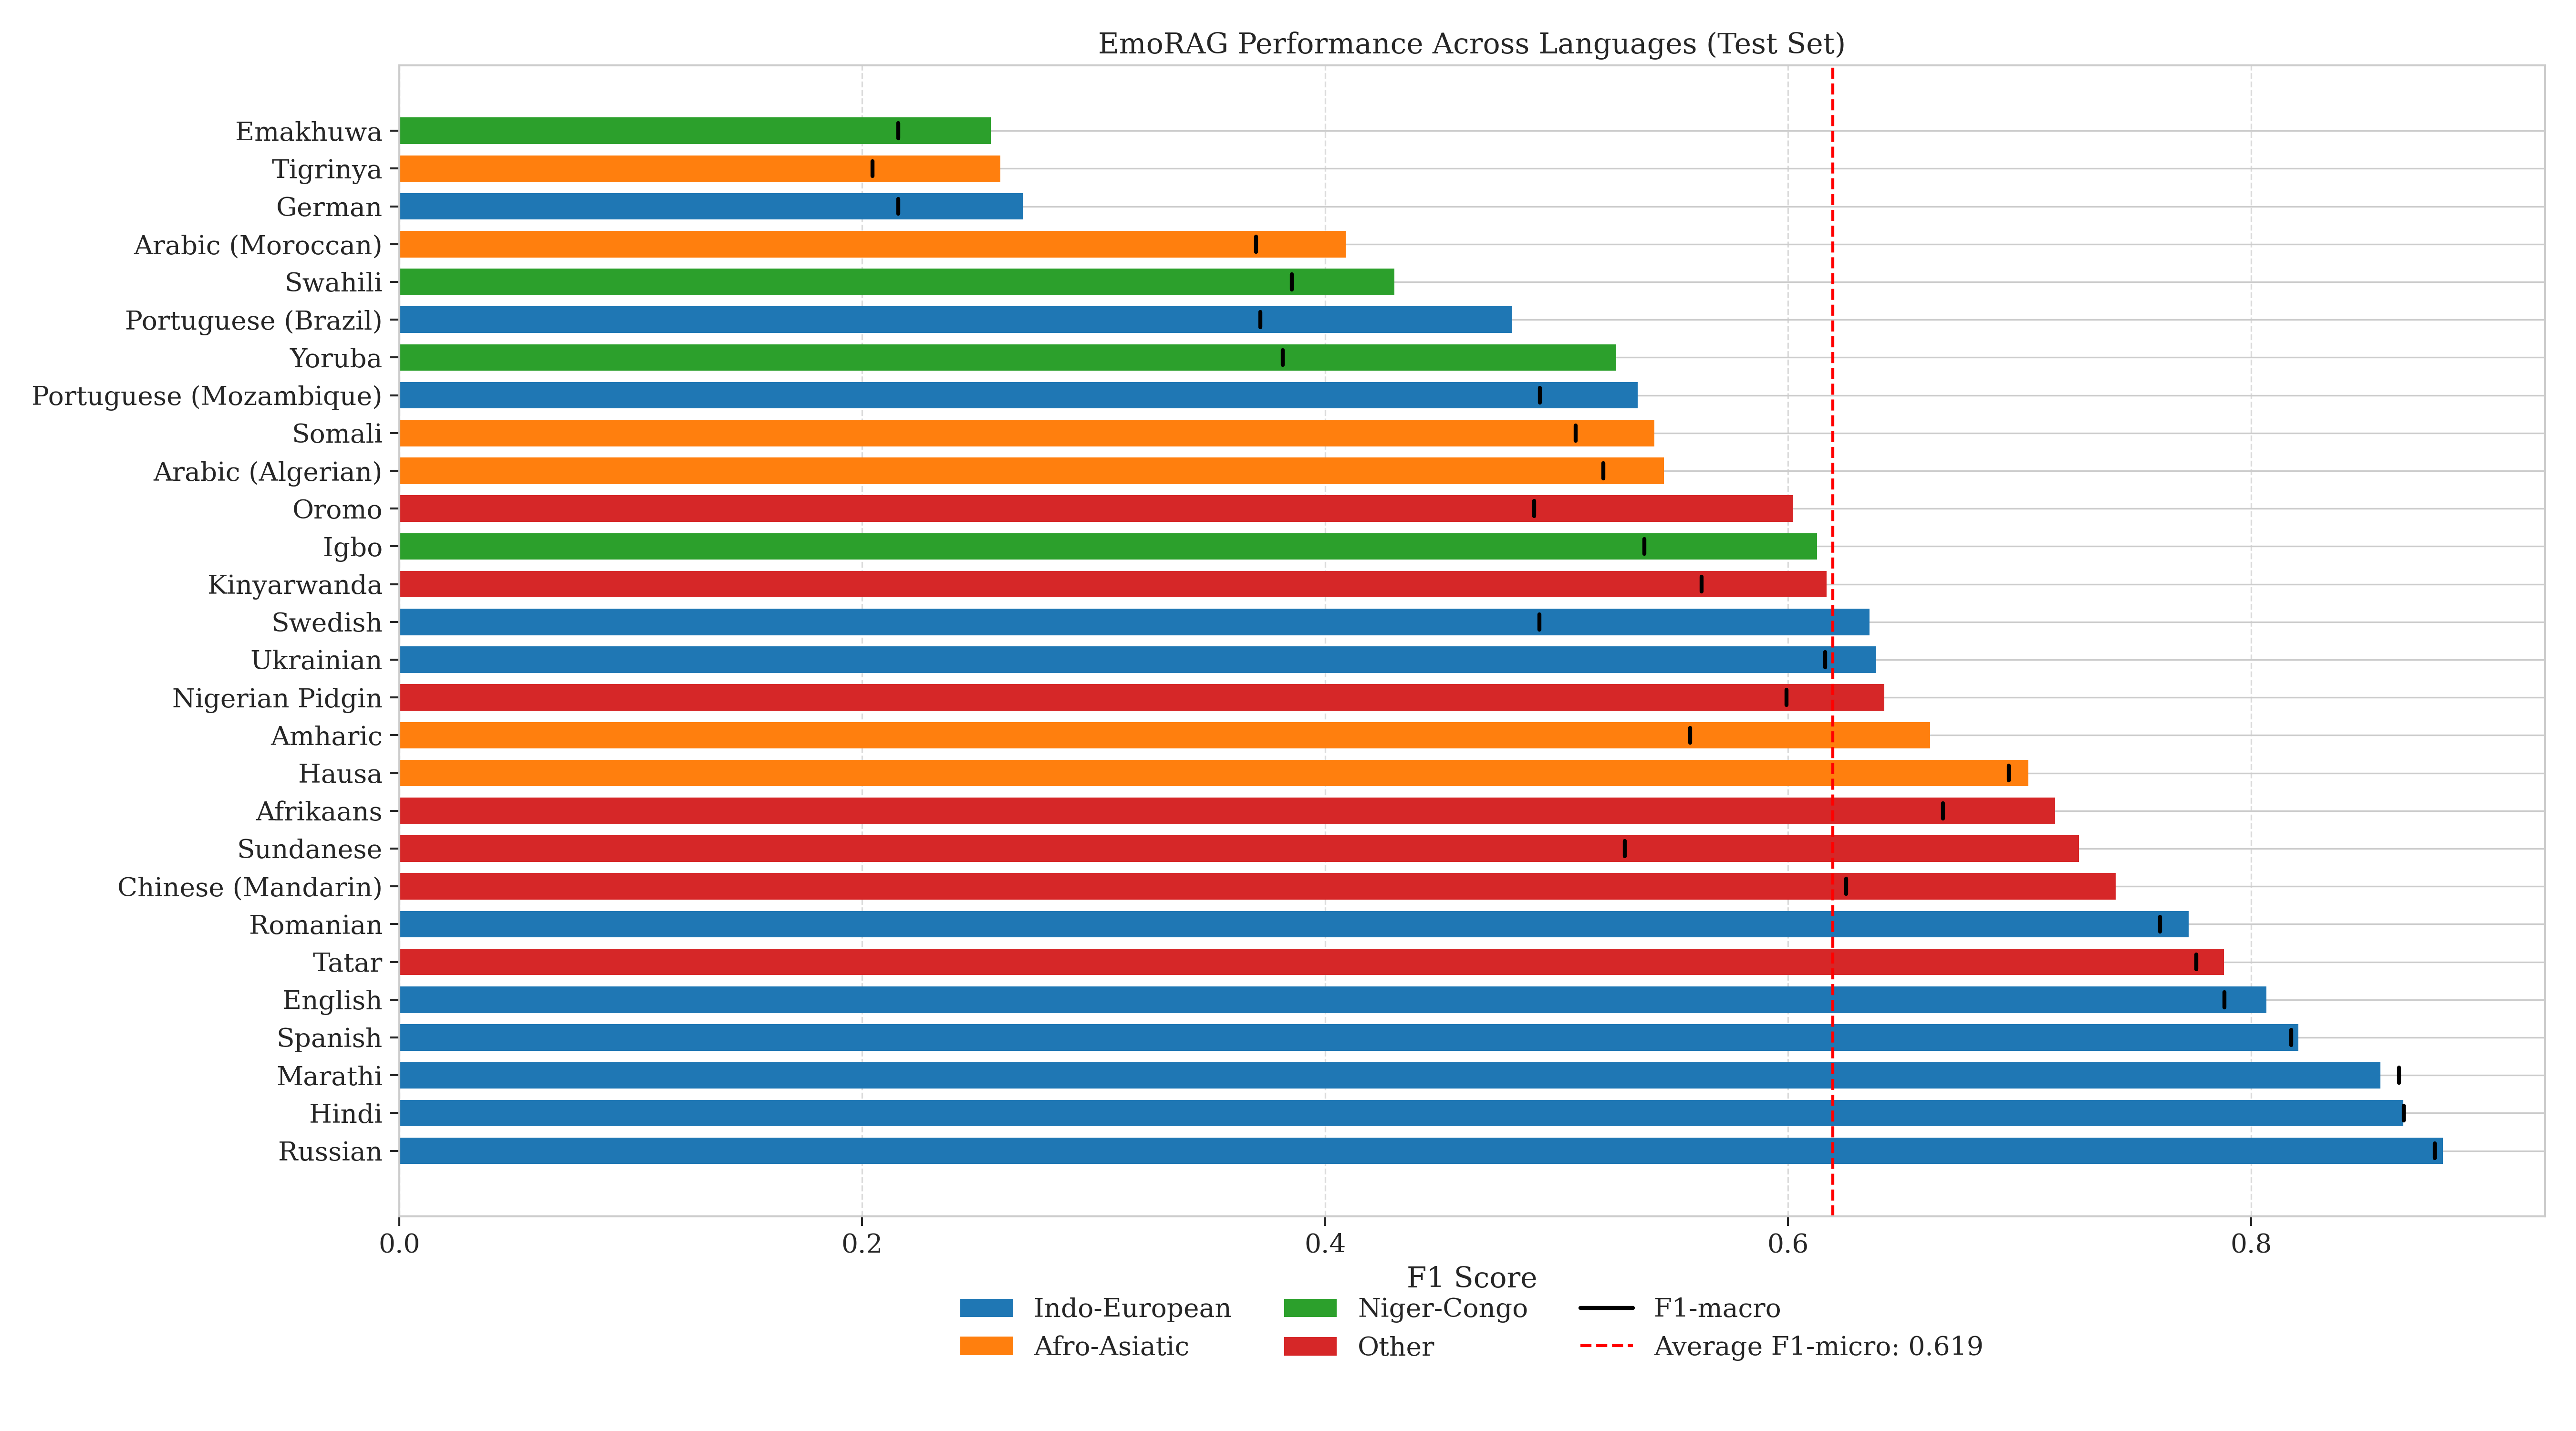
\includegraphics[width=1\textwidth]{emorag_by_language.png}
    \caption{EmoRAG performance across all 28 languages in the BRIGHTER dataset}
    \label{fig:emorag_by_language}
\end{figure}


Table \ref{tab:multilingual_performance} presents the performance of our best EmoRAG system across all 28 languages in the BRIGHTER dataset on the validation set, showing F1-micro/F1-macro scores for each language and aggregation method.

Table \ref{tab:test_metrics} presents the performance of our best EmoRAG system across all 28 languages in the BRIGHTER dataset on the test set, showing F1-micro/F1-macro scores for each language and aggregation method.

Figure \ref{fig:emorag_by_language} shows the performance of our best EmoRAG system across all 28 languages in the BRIGHTER dataset on the validation set, showing F1-micro/F1-macro scores for the best performing model for each language.

\begin{table*}[!th]
\begin{center}
    
    \footnotesize
    \resizebox{\textwidth}{!}{
    \begin{tabular}{@{}lccccccccc@{}}
    \toprule
    \textbf{Language} & \textbf{llama-3.1-70b} & \textbf{qwen2.5-70b} & \textbf{gpt-4o-mini} & \textbf{gpt-4o-mini-ngram} & \textbf{gemma29b} & \textbf{gemma29b\_ngram} & \textbf{majority\_vote} & \textbf{majority\_vote\_macro} & \textbf{majority\_vote\_by\_label\_f1} \\ \midrule
    amh & 0.534/0.448 & - & \textbf{0.637/0.503} & 0.633/0.493 & 0.609/0.488 & 0.582/0.474 & 0.659/0.535 & 0.659/0.535 & 0.655/0.539 \\
    arq & 0.584/0.575 & 0.623/0.597 & 0.613/0.596 & \textbf{0.663/0.655} & 0.614/0.589 & 0.578/0.531 & 0.645/0.615 & 0.653/0.665 & 0.687/0.677 \\
    ary & 0.542/0.490 & 0.540/0.485 & 0.552/0.499 & \textbf{0.576/0.512} & 0.575/0.521 & 0.584/0.484 & 0.607/0.526 & 0.526/0.599 & 0.616/0.540 \\
    afr & 0.560/0.444 & \textbf{0.629/0.527} & 0.662/0.567 & 0.646/0.572 & 0.584/0.481 & 0.484/0.398 & 0.601/0.494 & 0.546/0.646 & 0.662/0.557 \\
    chn & 0.676/0.603 & 0.589/0.570 & 0.698/0.579 & \textbf{0.748/0.604} & 0.693/0.572 & 0.709/0.543 & 0.749/0.642 & 0.652/0.757 & 0.759/0.659 \\
    deu & 0.745/0.588 & 0.521/0.499 & \textbf{0.745/0.694} & 0.738/0.662 & 0.632/0.559 & 0.659/0.593 & 0.738/0.659 & 0.672/0.741 & 0.752/0.695 \\
    eng & 0.735/0.726 & 0.779/0.775 & 0.807/0.803 & 0.770/0.781 & 0.769/0.759 & 0.720/0.723 & 0.801/0.808 & 0.813/0.810 & \textbf{0.821/0.818} \\
    esp & 0.751/0.744 & 0.788/0.778 & 0.793/0.785 & 0.799/0.793 & 0.778/0.772 & 0.782/0.778 & 0.786/0.778 & 0.807/0.812 & \textbf{0.813/0.809} \\
    hau & 0.610/0.602 & 0.607/0.598 & 0.669/0.662 & \textbf{0.696/0.687} & 0.682/0.676 & 0.698/0.689 & 0.735/0.728 & 0.734/0.738 & 0.735/0.731 \\
    hin & 0.780/0.791 & 0.707/0.728 & 0.805/0.803 & 0.811/0.812 & 0.796/0.799 & 0.798/0.806 & 0.838/0.842 & 0.833/0.830 & \textbf{0.842/0.849} \\
    ibo & 0.531/0.486 & 0.502/0.452 & 0.572/0.514 & 0.564/0.499 & 0.574/0.508 & 0.574/0.520 & 0.609/0.532 & 0.534/0.608 & \textbf{0.614/0.550} \\
    kin & 0.443/0.385 & 0.443/0.382 & 0.555/0.491 & \textbf{0.576/0.489} & 0.477/0.404 & 0.514/0.466 & 0.589/0.515 & 0.501/0.570 & 0.575/0.512 \\
    mar & 0.874/0.883 & 0.904/0.908 & 0.937/0.939 & 0.937/0.939 & 0.883/0.883 & 0.897/0.900 & 0.942/0.946 & 0.935/0.931 & \textbf{0.943/0.947} \\
    orm & 0.467/0.369 & 0.521/0.415 & 0.552/0.455 & \textbf{0.607/0.501} & 0.519/0.404 & 0.488/0.362 & 0.585/0.446 & 0.493/0.608 & 0.608/0.488 \\
    pcm & 0.532/0.508 & 0.573/0.535 & 0.599/0.542 & \textbf{0.628/0.573} & 0.608/0.572 & 0.585/0.548 & 0.621/0.574 & 0.590/0.633 & 0.638/0.591 \\
    ptbr & 0.686/0.547 & 0.662/0.569 & 0.731/0.633 & 0.707/0.603 & 0.726/0.617 & 0.710/0.525 & 0.766/0.626 & 0.658/0.760 & \textbf{0.766/0.645} \\
    ptmz & 0.454/0.456 & 0.539/0.532 & 0.515/0.484 & 0.478/0.443 & 0.521/0.486 & 0.494/0.445 & 0.565/0.558 & 0.543/0.552 & \textbf{0.565/0.558} \\
    ron & 0.758/0.749 & 0.745/0.726 & 0.756/0.741 & 0.778/0.763 & 0.745/0.719 & 0.754/0.724 & 0.773/0.751 & 0.771/0.790 & \textbf{0.794/0.774} \\
    rus & 0.835/0.836 & 0.861/0.857 & 0.839/0.833 & 0.812/0.806 & 0.841/0.834 & 0.824/0.817 & 0.879/0.877 & 0.881/0.883 & \textbf{0.880/0.880} \\
    som & 0.361/0.296 & 0.379/0.338 & 0.518/0.469 & 0.528/0.491 & 0.426/0.381 & 0.428/0.382 & 0.494/0.420 & 0.464/0.514 & \textbf{0.519/0.477} \\
    sun & 0.674/0.496 & 0.707/0.491 & 0.734/0.596 & 0.757/0.612 & 0.708/0.532 & 0.733/0.565 & 0.754/0.537 & 0.564/0.750 & \textbf{0.757/0.614} \\
    swa & 0.357/0.329 & 0.376/0.345 & 0.391/0.366 & 0.416/0.401 & 0.401/0.366 & 0.407/0.372 & 0.435/0.396 & 0.401/0.435 & \textbf{0.440/0.409} \\
    swe & 0.684/0.475 & 0.680/0.502 & 0.709/0.528 & 0.708/0.529 & 0.699/0.518 & 0.671/0.501 & 0.734/0.555 & 0.547/0.727 & \textbf{0.736/0.582} \\
    tat & 0.652/0.611 & 0.663/0.631 & 0.712/0.671 & 0.702/0.660 & 0.669/0.634 & 0.637/0.592 & 0.727/0.673 & 0.688/0.732 & \textbf{0.749/0.710} \\
    tir & - & - & 0.377/0.321 & 0.384/0.319 & - & - & 0.322/0.263 & 0.321/0.377 & \textbf{0.397/0.342} \\
    ukr & 0.521/0.512 & 0.601/0.579 & 0.581/0.567 & 0.550/0.537 & 0.587/0.553 & 0.535/0.469 & 0.622/0.611 & 0.621/0.625 & \textbf{0.634/0.621} \\
    vmw & 0.158/0.145 & 0.261/0.184 & 0.300/0.211 & 0.226/0.158 & 0.246/0.206 & 0.186/0.159 & 0.190/0.140 & 0.180/0.230 & \textbf{0.257/0.205} \\
    yor & 0.354/0.255 & 0.415/0.300 & 0.474/0.374 & 0.506/0.420 & 0.436/0.317 & 0.472/0.347 & 0.564/0.443 & 0.423/0.532 & \textbf{0.564/0.443} \\ \midrule
    \textbf{Average} & \textbf{0.563/0.515} & \textbf{0.590/0.556} & \textbf{0.631/0.590} & \textbf{0.641/0.601} & \textbf{0.617/0.576} & \textbf{0.607/0.566} & \textbf{0.661/0.617} & \textbf{0.646/0.634} & \textbf{0.678/0.634} \\ \bottomrule
    \end{tabular}
    }
\end{center}
\caption{Development set F1-micro/F1-macro scores for each language and model. The best model for each language is highlighted in bold.}
\label{tab:multilingual_performance}
\end{table*}

\begin{table*}[th!]
\centering
\footnotesize

\resizebox{.99\textwidth}{!}{

\begin{tabular}{@{}lcccccc@{}}
\toprule
\textbf{Language} & \textbf{Language Code} & \textbf{Best Model} & \textbf{Dev F1 Micro} & \textbf{Dev F1 Macro} & \textbf{Test F1 Micro} & \textbf{Test F1 Macro} \\ \midrule
Afrikaans & afr & majority\_vote\_by\_label\_f1 & 0.662 & 0.557 & 0.7153 & 0.667 \\
Amharic & amh & gpt-4o-mini & 0.637 & 0.503 & 0.6613 & 0.5578 \\
German & deu & gpt-4o-mini & 0.745 & 0.694 & 0.2694 & 0.2156 \\
English & eng & majority\_vote\_by\_label\_f1 & 0.821 & 0.818 & 0.8066 & 0.7885 \\
Spanish & esp & majority\_vote\_by\_label\_f1 & 0.813 & 0.809 & 0.8204 & 0.8174 \\
Hindi & hin & majority\_vote\_by\_label\_f1 & 0.842 & 0.849 & 0.8658 & 0.8661 \\
Marathi & mar & majority\_vote\_by\_label\_f1 & 0.943 & 0.947 & 0.8559 & 0.864 \\
Oromo & orm & gpt-4o-mini-ngram & 0.607 & 0.501 & 0.6023 & 0.4903 \\
Portuguese (Brazil) & ptbr & majority\_vote\_by\_label\_f1 & 0.766 & 0.645 & 0.4809 & 0.372 \\
Russian & rus & majority\_vote\_by\_label\_f1 & 0.880 & 0.880 & 0.8829 & 0.8794 \\
Somali & som & majority\_vote\_by\_label\_f1 & 0.519 & 0.477 & 0.5422 & 0.5082 \\
Sundanese & sun & gpt-4o-mini-ngram & 0.757 & 0.612 & 0.7256 & 0.5294 \\
Tatar & tat & majority\_vote\_by\_label\_f1 & 0.749 & 0.710 & 0.7884 & 0.7763 \\
Tigrinya & tir & majority\_vote\_by\_label\_f1 & 0.397 & 0.342 & 0.2597 & 0.2044 \\
Arabic (Algerian) & arq & majority\_vote\_by\_label\_f1 & 0.687 & 0.677 & 0.5464 & 0.5203 \\
Arabic (Moroccan) & ary & gpt-4o-mini-ngram & 0.576 & 0.512 & 0.4089 & 0.3701 \\
Chinese (Mandarin) & chn & gpt-4o-mini-ngram & 0.748 & 0.604 & 0.7416 & 0.6252 \\
Hausa & hau & majority\_vote\_by\_label\_f1 & 0.735 & 0.731 & 0.7039 & 0.6954 \\
Kinyarwanda & kin & gpt-4o-mini-ngram & 0.576 & 0.489 & 0.6167 & 0.5627 \\
Nigerian Pidgin & pcm & majority\_vote\_by\_label\_f1 & 0.638 & 0.591 & 0.6416 & 0.5993 \\
Portuguese (Mozambique) & ptmz & majority\_vote\_by\_label\_f1 & 0.565 & 0.558 & 0.535 & 0.4927 \\
Swahili & swa & majority\_vote\_by\_label\_f1 & 0.440 & 0.409 & 0.43 & 0.3856 \\
Swedish & swe & majority\_vote\_by\_label\_f1 & 0.736 & 0.582 & 0.6353 & 0.4926 \\
Ukrainian & ukr & majority\_vote\_by\_label\_f1 & 0.634 & 0.621 & 0.638 & 0.6161 \\
Emakhuwa & vmw & gpt-4o-mini & 0.300 & 0.211 & 0.2556 & 0.2157 \\
Yoruba & yor & majority\_vote\_by\_label\_f1 & 0.564 & 0.443 & 0.5257 & 0.3818 \\
Igbo & ibo & majority\_vote\_by\_label\_f1 & 0.614 & 0.550 & 0.6125 & 0.5379 \\
Romanian & ron & majority\_vote\_by\_label\_f1 & 0.794 & 0.774 & 0.773 & 0.7608 \\ \midrule
\textbf{Average} & & & & & \textbf{0.638} & \textbf{0.590} \\ \bottomrule
\end{tabular}
}
\caption{Test set performance metrics for each language using the best model according to the development dataset results.}
\label{tab:test_metrics}
\end{table*}


Our analysis revealed several important patterns:

\begin{itemize}
\item \textbf{High-resource vs. Low-resource Languages}: High-resource languages like English (0.821/0.818), Russian (0.880/0.880), and Hindi (0.842/0.849) consistently achieved the highest performance across all approaches. Low-resource languages like Tigrinya (0.397/0.342), Swahili (0.440/0.409), and Makhuwa (0.257/0.205) showed significantly lower performance, with F1 scores often below 0.5.

\item \textbf{Language Family Analysis}: We observed performance clusters within language families. Indo-European languages (English, German, Spanish, Romanian) consistently performed well, with an average F1-micro of 0.795. Niger-Congo languages (Yoruba, Igbo, Swahili) showed more variable performance, with an average F1-micro of 0.563. Afro-Asiatic languages (Amharic, Tigrinya) generally performed below average, with F1-micro scores around 0.526.

\item \textbf{Retrieval Strategy Impact}: For some languages, particularly those with unique scripts or limited representation in pre-training data, n-gram retrieval outperformed embedding-based retrieval. This was evident in Oromo (0.607 vs. 0.552), Moroccan Arabic (0.576 vs. 0.552), and Chinese (0.748 vs. 0.698).

\item \textbf{Aggregation Strategy Effectiveness}: The label-specific F1 weighting strategy proved most effective overall, outperforming other aggregation methods in 17 out of 28 languages. This suggests that emotion-specific expertise varies across models and languages, and weighting predictions accordingly yields better results.
\end{itemize}


\section{Ablation Studies}

To understand the contribution of different components to EmoRAG's performance, we conducted extensive ablation studies.

\subsection{EmoRAG Components}

\begin{table}[h]
\centering
\begin{tabular}{lcc}
\toprule
\textbf{Component Configuration} & \textbf{F1-micro} & \textbf{F1-macro} \\
\midrule
Full EmoRAG system & 0.678 & 0.634 \\
Without embedding retriever & 0.641 & 0.601 \\
Without n-gram retriever & 0.631 & 0.590 \\
Without label-specific weighting & 0.661 & 0.617 \\
Single model (GPT-4o-mini) & 0.631 & 0.590 \\
\bottomrule
\end{tabular}
\caption{Ablation study of EmoRAG components (averaged across all languages)}
\label{tab:ablation_components}
\end{table}

Removing the embedding-based retriever reduced performance by 5.5\% on average, with larger impacts on high-resource languages. Removing the n-gram retriever had a smaller overall impact (6.9\% reduction) but significantly affected low-resource languages with unique scripts. The label-specific weighting strategy contributed a 2.6\% improvement over simple majority voting, with larger gains in languages with imbalanced emotion distributions.

\subsection{Example Count Analysis}

% \begin{figure}[h]
%     \centering
%     \includegraphics[width=0.8\textwidth]{example_count_analysis.png}
%     \caption{Performance vs. number of retrieved examples}
%     \label{fig:example_count}
% \end{figure}

We varied the number of retrieved examples (K) from 0 to 1000 and found that performance generally improved with more examples up to a point, after which returns diminished or performance decreased. The optimal K varied by language: high-resource languages benefited from larger K values (100-150), while low-resource languages performed best with moderate K values (30-50). This suggests that quality of examples matters more than quantity for low-resource settings.

\begin{table}[h]
\centering
\begin{tabular}{lcc}
\toprule
\textbf{Number of Examples (K)} & \textbf{F1-micro} & \textbf{F1-macro} \\
\midrule
0 (zero-shot) & 0.5959 & 0.6164 \\
30 & 0.8036 & 0.8001 \\
100 & 0.8071 & 0.8026 \\
300 & 0.7911 & 0.7762 \\
1000 & 0.7882 & 0.7769 \\
\bottomrule
\end{tabular}
\caption{Impact of retrieved example count on GPT-4o-mini performance for English language}
\label{tab:example_count}
\end{table}

As shown in Table \ref{tab:example_count}, for English, performance improves dramatically when moving from zero-shot to few-shot with 30 examples, with a slight additional improvement at 100 examples. However, increasing to 300 or 1000 examples actually leads to decreased performance. This pattern suggests that there is an optimal window for the number of retrieved examples, beyond which the model may become overwhelmed with potentially conflicting information or less relevant examples.

\subsection{Cross-model Analysis}

\begin{table}[h]
\centering
\begin{tabular}{lcc}
\toprule
\textbf{Model} & \textbf{F1-micro} & \textbf{F1-macro} \\
\midrule
GPT-4o-mini & 0.631 & 0.590 \\
Llama-3.1-70B & 0.649 & 0.612 \\
Qwen2.5-72B & 0.657 & 0.621 \\
Gemma-2-27B & 0.618 & 0.583 \\
All models (ensemble) & 0.678 & 0.634 \\
\bottomrule
\end{tabular}
\caption{Performance comparison across different LLMs (averaged across all languages)}
\label{tab:cross_model}
\end{table}

Each model in our ensemble showed different strengths across languages and emotions. Llama-3.1-70B performed best on Germanic and Romance languages, while Qwen2.5-72B excelled on Asian languages. GPT-4o-mini showed more balanced performance across the board. Gemma-2-27B, despite its smaller size, contributed valuable predictions for specific emotion-language combinations, particularly for surprise and fear in Slavic languages.

The ensemble consistently outperformed individual models, with an average improvement of 3.2\% in F1-micro score over the best single model. This confirms the complementary nature of different LLMs' knowledge and the effectiveness of our aggregation strategies in leveraging their combined strengths.

\section{Discussion}

Our evaluation of different approaches to multilingual, multi-label emotion detection reveals several important insights about the strengths, limitations, and practical considerations of each method.

\subsection{Comparison of Approaches}

The experimental results demonstrate clear performance differences between traditional supervised approaches and our retrieval-augmented generation system. Each approach offers distinct advantages and limitations:

\textbf{BERT-based Approach:} While providing a strong baseline (F1-micro of 0.7145 on English), this approach requires substantial labeled data for each language and emotion category. Its performance degrades significantly for low-resource languages where pre-training data is limited. The main advantage is its inference efficiency (0.05 seconds per sample), making it suitable for real-time applications with deployment constraints.

\textbf{SetFit Approach:} This few-shot learning technique (F1-micro of 0.6943 on English) offers a good balance between data efficiency and performance. It requires less training data than BERT but still needs some labeled examples for each language. SetFit's contrastive learning stage helps capture semantic relationships between texts expressing similar emotions, but it struggles with the multi-label aspect of emotion detection.

\textbf{Seq2Seq Approach:} Despite its theoretical appeal for handling label dependencies, this approach showed the weakest performance among supervised methods (F1-micro of 0.5126 on English). The generative framing of emotion detection appears less effective than discriminative approaches, possibly due to the challenge of generating precise combinations of emotion labels.

\textbf{EmoRAG System:} Our novel retrieval-augmented approach achieved the highest performance across languages (F1-micro of 0.821 on English, 0.678 average across all languages). Its key strength is adaptability to new languages without requiring model retraining, making it particularly valuable for low-resource scenarios. 
The main drawback is higher inference cost due to multiple LLM calls (2.5 seconds per sample with four models).
However, experiments show that using a single model (for example, gpt-4o-mini) is still better than any other experimented supervised approach.

\subsection{Performance on Low-resource Languages}

Our results highlight persistent challenges in emotion detection for low-resource languages. The performance disparity between high-resource languages like English (F1-micro of 0.821) and low-resource languages like Makhuwa (F1-micro of 0.257) remains substantial.

Several factors contribute to these challenges:

\textbf{Script and Tokenization Issues:} Languages with unique scripts or limited representation in pre-training data face tokenization challenges that affect model performance. This explains why n-gram retrieval outperformed embedding-based retrieval for languages like Oromo, Moroccan Arabic, and Chinese.

\textbf{Cultural Expression of Emotions:} Emotions are expressed differently across cultures, and these nuances may not be well-captured in models primarily trained on high-resource languages. The ablation studies showed that increasing the number of retrieved examples beyond a certain point (30-50 for low-resource languages) actually decreased performance, suggesting that quality and relevance of examples matter more than quantity.

\subsection{Error Analysis with Examples}

Analysis of misclassifications reveals several common error patterns across approaches, which can be illustrated through specific examples from our evaluation dataset:

\textbf{Emotion Intensity Confusion:} All approaches struggled with distinguishing between different intensities of the same emotion. For example, as shown in Table~\ref{tab:intensity-confusion}:

\begin{table}[h]
\centering
\begin{tabular}{|p{8.5cm}|p{2.5cm}|p{2.5cm}|}
\hline
\textbf{Text} & \textbf{True Emotions} & \textbf{Predicted Emotions} \\
\hline
``Ich wurde mit 17 ins Milieu verschleppt, gehandelt, verkauft, zur einer Schwangerschaft (und Austragung) gezwungen und konnte erst mit fast 20 flüchten. Gemeinsam mit meinem Kind.'' \newline (German: "I was abducted into prostitution at 17, trafficked, sold, forced into pregnancy (and carrying to term) and could only escape at almost 20. Together with my child.") & anger, disgust, sadness & anger, disgust, fear, sadness \\
\hline
``Taurus-Leaks: Der Skandal besteht darin, dass deutsche Offiziere mit deutschen Waffen einen Angriff gegen Russland bis ins Detail planen.'' \newline (German: "Taurus Leaks: The scandal is that German officers are planning an attack against Russia with German weapons in detail.") & anger, disgust, fear & anger, disgust, fear, surprise \\
\hline
\end{tabular}
\caption{Examples of emotion intensity confusion}
\label{tab:intensity-confusion}
\end{table}

In these examples, the model correctly identified the primary emotions but added additional emotions that weren't annotated, suggesting difficulty in calibrating emotional intensity thresholds.

\textbf{Cultural Nuances:} Expressions that rely on cultural context or idioms were frequently misclassified, as illustrated in Table~\ref{tab:cultural-nuances}:

\begin{table}[h]
\centering
\begin{tabular}{|p{8.5cm}|p{2.5cm}|p{2.5cm}|}
\hline
\textbf{Text} & \textbf{True Emotions} & \textbf{Predicted Emotions} \\
\hline
``@<username> @<username> Jack na akpari onwe ya'' \newline (Igbo: "Jack is just boasting") & anger & [none] \\
\hline
``Anu Matak Mun di Imah kosong tong ngomong punten bisi Aya NU nembalan'' \newline (Sundanese: "Why do we say 'excuse me' in an empty house? In case someone answers") & fear & fear, surprise \\
\hline
``Vi blev någorlunda nöjda. Vi kommenterade missnöjet, en väldigt liten åtgärd gjordes men ändock blev vi inte helt nöjda.'' \newline (Swedish: "We were somewhat satisfied. We commented on the dissatisfaction, a very small measure was taken but still we were not completely satisfied.") & joy & anger, sadness \\
\hline
\end{tabular}
\caption{Examples of cultural nuance misclassifications}
\label{tab:cultural-nuances}
\end{table}

These examples demonstrate how culturally-specific expressions of emotions can be misinterpreted, particularly in low-resource languages where models have less exposure to cultural nuances.

\textbf{Co-occurring Emotions:} Cases where multiple emotions co-occur presented challenges, as shown in Table~\ref{tab:co-occurring-emotions}:

\begin{table}[h]
\centering
\begin{tabular}{|p{8.5cm}|p{2.5cm}|p{2.5cm}|}
\hline
\textbf{Text} & \textbf{True Emotions} & \textbf{Predicted Emotions} \\
\hline
``It overflowed and brown shitty diarrhea water came flooding under the stall wall into my wife's stall.'' & anger, fear, sadness, surprise & anger, fear, surprise \\
\hline
``Caz halucinant de cruzime Un bărbat acuză un polițist din Sibiu că la snopit în bătaie "Am stat în genunchi"'' \newline (Romanian: "Hallucinating case of cruelty A man accuses a police officer from Sibiu of beating him up 'I was on my knees'") & anger, disgust, fear, sadness, surprise & anger, disgust, sadness \\
\hline
``Pobre chica, te quemaste tu solita.'' \newline (Spanish: "Poor girl, you burned yourself.") & disgust, sadness, surprise & sadness \\
\hline
\end{tabular}
\caption{Examples of co-occurring emotion misclassifications}
\label{tab:co-occurring-emotions}
\end{table}

These examples show that models often capture the dominant emotions but miss secondary or tertiary emotions, particularly in complex emotional scenarios.

\textbf{Linguistic Structure:} Languages with significantly different syntactic structures showed higher error rates, as demonstrated in Table~\ref{tab:linguistic-structure}:

\begin{table}[h]
\centering
\begin{tabular}{|p{8.5cm}|p{2.5cm}|p{2.5cm}|}
\hline
\textbf{Text} & \textbf{True Emotions} & \textbf{Predicted Emotions} \\
\hline
``[Tigrinya text omitted]'' \newline (Tigrinya expression of disgust) & disgust & [none] \\
\hline
``[Makhuwa text omitted]'' \newline (Makhuwa: "Brazil is now the father of the World Cup and looks weak.") & sadness & [none] \\
\hline
``[Chinese text omitted]'' \newline (Chinese: "Sigh, people can't see that he's still the pill king, don't know where he got the money from, I'm short on cash recently and would like to earn some too.") & [none] & anger \\
\hline
\end{tabular}
\caption{Examples of linguistic structure challenges}
\label{tab:linguistic-structure}
\end{table}

These examples highlight the challenges in processing languages with different scripts and syntactic structures, particularly for low-resource languages where pre-training data is limited.

\section{Conclusions}

This thesis has investigated various approaches for multilingual, multi-label emotion detection, with a particular focus on addressing the challenges of low-resource languages. We compared traditional supervised approaches (BERT, SetFit, and Seq2Seq) with a novel retrieval-augmented generation system (EmoRAG). We have evaluated our system on 28 languages from the BRIGHTER dataset.

\subsection{Summary of Findings}

Our research has yielded several key findings:

\begin{itemize}
    \item Retrieval-augmented generation significantly outperforms traditional supervised approaches for emotion detection on English, with our EmoRAG system achieving an average F1-micro score of 0.678 across all languages compared to 0.715 for the best supervised approach (BERT).
    
    \item The performance gap between high-resource and low-resource languages still remains substantial.
    
    \item Different retrieval strategies are optimal for different languages: embedding-based retrieval works best for high-resource languages with substantial pre-training data, while n-gram retrieval often performs better for languages with unique scripts or limited representation in pre-training.
    
    \item Ensemble methods that combine predictions from multiple models with label-specific weighting strategies consistently outperformed single-model approaches, demonstrating the complementary nature of different LLMs' capabilities across languages and emotions.
    
\end{itemize}

\subsection{Limitations}

Despite the promising results, our approaches face several limitations:

\begin{itemize}
    \item Performance on Very Low-Resource Languages: Even with retrieval augmentation, performance on extremely low-resource languages like Makhuwa (F1-micro of 0.257) and Tigrinya (F1-micro of 0.397) remained poor, indicating that fundamental challenges in cross-lingual transfer persist.
    
    \item Cultural Nuance: All approaches struggled with culturally-specific expressions of emotion, particularly idioms and metaphorical language that require cultural context to interpret correctly.
    
    \item Retrieval Quality: The effectiveness of retrieval-augmented approaches depends heavily on the quality and relevance of retrieved examples. Current retrieval mechanisms do not account for cultural or pragmatic factors that influence emotion expression.
    
\end{itemize}


In conclusion, while there are still challenges in detecting emotions across multiple languages, especially those with fewer resources, our research shows that using retrieval-augmented methods is a promising way forward. By leveraging the capabilities of large language models and flexible retrieval techniques, we can create systems that better understand emotions in different cultural contexts.

Our EmoRAG system participated in the SemEval2025-Task11 competition, ranking in the top 10 on average across all languages, with some languages achieving top 3 performance. 

EmoRAG system description paper was accepted at the ACL Workshop 2025.

We have made our complete implementation publicly available at \url{https://github.com/galthran-wq/semeval25-text-emotions}. This repository includes code for all components of the EmoRAG system and the complete implementation of all approaches tested in this thesis.

\printbibliography

\appendix


% \section{LLM Prompt for Emotion Detection} 
% \label{appendix:llm_prompt}

% \lstset{
%   basicstyle=\small\ttfamily,
%   breaklines=true,
%   breakatwhitespace=false,
%   breakindent=0pt,
%   literate={-}{{-}}1, % ensures hyphens are treated properly
% }

% The following prompt is used to instruct the language model for perceived emotion detection:

% \begin{tcolorbox}[
%   colback=orange!5, 
%   colframe=orange!90!black, 
%   fonttitle=\bfseries, 
%   title=Emotion Detection Prompt, 
%   boxrule=1pt, 
%   arc=4pt, 
%   auto outer arc, 
%   boxsep=5pt, 
%   left=5pt, 
%   right=5pt, 
%   top=5pt, 
%   bottom=5pt, 
%   halign=justify,
%   width=0.95\textwidth
% ]
% \begin{lstlisting}
% You are an expert at detecting emotions in text. The texts are given in {language} language.
% Please classify the text into one of the following categories:
% Anger, Fear, Joy, Sadness, Surprise, Disgust
% Your response should be a JSON object with the following format:
% {
%     "anger": bool,
%     "fear": bool,
%     "joy": bool,
%     "sadness": bool,
%     "surprise": bool,
%     "disgust": bool
% }
% Do not give explanations. Just return the JSON object.
% \end{lstlisting}
% \end{tcolorbox}


\end{document}
